
\documentclass[\PRJWD/Thick_TQFTs_and_Quantum_Information.tex]{subfiles}

\begin{document}

\section{Introduction}

The monoidal category $2\Thick$ of thick tangles is the monoidal category freely
generated by the composition of the following morphisms \cite{NonCommTQFT}:
\[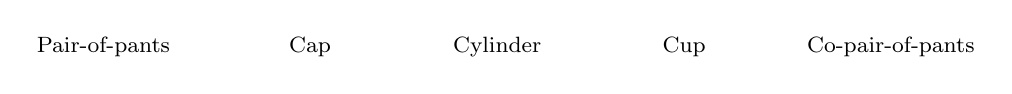
\begin{tikzpicture}[scale=0.25]
\pants{0, 0}
\node at (0, -5) {\footnotesize Pair-of-pants};
\capcob{12, 0}
\node at (10.5, -5) {\footnotesize Cap};
\idcob{20, 0}
\node at (20, -5) {\footnotesize Cylinder};
\cupcob{28, 0}
\node at (29.5, -5) {\footnotesize Cup};
\copants{40, 0}
\node at (40, -5) {\footnotesize Co-pair-of-pants};
\end{tikzpicture}\]
Consider a planar open string topological quantum field theory
$F : 2\Thick \to \Vect_{\C}$ as defined in \cite{NonCommTQFT}. $F$ is
determined by the images of the above generating structures under $F$. One
possible to way to connect quantum information to topological quantum
field theories is to assume that the image of the interval $I$ under $F$
is some finite dimensional $C^*$--algebra of operators on some Hilbert space of
states. Coecke, Heunen and Kissinger \cite{CatQChan} have shown that every such
algebra is, in fact, a dagger Frobenius algebra, with some additional structure,
so that this assumption on $F$ is valid. In fact, every finite dimensional
$C^*$--algebra arises as the image of the interval under such a planar open
string field theory.

It is well-known that finite dimensional $C^*$--algebras, up to
$*$--isomorphism, are finite direct sums of square matrix algebras $\bigoplus_i
\M_{n_i}$ where $\M_n$ is the set of $n \times n$ matrices with complex entries
equipped with the usual multiplication. For simplicity, we first assume that
$F(I)$ is the $C^*$--algebra $\M_n$. Then, we can consider quantum gates to be
elements of $\M_n$ and circuits to be composites (products) of these
elements. While $\M_n$ has all gates necessary for quantum computing for some
fixed number of qubits, there is a major constraint on the elements of $\M_n$
that are in the image of $F$, as we describe below.

Elements $a \in \M_n$ can be seen as maps $\C \to \M_n : z \mapsto za$. The
elements that are accounted for by $F$ are images of thick tangles
$\varnothing \to I$. However, these ``element'' thick tangles are determined by
their genus, since in $2\Thick$ we identify morphisms up to diffeomorphism, so
that all element thick tangles must decompose as follows:
\[\begin{tikzpicture}[scale=0.25]
\cupcob{0, 0}
\copants{4, 0}
\pants{8, 0}
\copants{12, 0}
\pants{16, 0}
\draw[loosely dotted, thick] (18.5, 0) -- (21.5, 0);
\copants{24, 0}
\pants{28, 0}
\end{tikzpicture}\]
where we take the domain of the thick tangle to be on the left and the codomain,
on the right. Call this thick tangle $R$. Let $m : \M_n \tensor \M_n \to \M_n$
be the multiplication of $\M_n$.  Then the multiplicative unit is
$e : \C \to \M_n : z \mapsto zI_n$ and, by the definition of dagger Frobenius
algebra, the comultiplication of $\M_n$ is $m^{\dagger}$. Hence, under $F$, the
element thick tangle above yields a map $(mm^{\dagger})^k e$, where
the superscript $k$ denotes a $k$--fold composite for some non-negative integer
$k$. Now, $mm^{\dagger}$ is the map $a \mapsto na$ \cite[10]{CatQChan}
so that
\[
  F(R)(z) = z \cdot F(R)(1) = z \cdot (mm^{\dagger})^ke(1) = zn^{k}I_n
\]

This shows that the only elements, in the usual sense of elements of $\M_n$,
that are accessible through $F$ are multiples of the identity matrix by powers
of $n$. It is then easy to see that for direct sums such as
$\bigoplus_{i = 1}^{q} \M_{n_i}$, the only accessible elements are
\[
  (n_1^k I_{n_1}, \dots, n_q^k I_{n_q})
\]
so that up to $*$--isomorphism, there are some major constraints on the quantum
gates that are accessible through planar open string field theories.
We note that this situation is brought about by the identification of thick
tangles up to diffeomorphisms. This motivates us to look for methods in a
setting where we drop this identification -- higher categories of thick tangles
(for instance, $\PTT$ as defined in \cite{NonSemiSimp}) (or cobordisms)
where gluing is associative and unital up to higher isomorphisms. We will
see that it suffices to consider double categories for obtaining a reasonable
method for formulating quantum information in terms of topological field
theories.

Recall that a monoidal double category consists of a $1$--category of objects
and a $1$--category of morphisms with source, target and unit functors, a notion
of horizontal composition of morphisms, and a monoidal structure on the object
and morphism categories. In addition, horizontal composition and monoidal
products need to be associative and unital up to isomorphism with several
coherence and compatibility properties \cite{SymMonBicat}. In this work,
however, by ``monoidal double category'' we will mean only the data of such a
structure. Nevertheless, wherever possible, we have commented on how the data of
our constructions inherit most of the necessary properties from the usual
categories of sets, manifolds, vector spaces, etc. Thus, we will construct
several monoidal double categories in this work but they should be seen as
monoidal double categories in a somewhat relaxed sense -- they consist of all
the required data but satisfy the required axioms with a few possible
exceptions. We will treat monoidal double functors in the same loose sense.

\end{document}

